\chapter{Analysis}

This section aims to apply the knowledge gained from the previous sections to the example of Bosch. Bosch is a engineering and technology company founded by Robert Bosch in Stuttgart in 1886. The Bosch Group is divided into several business sectors, namely Mobility, Consumer Goods, Industrial Technology and Building Technology, adding up to a total revenue of 90,3 Billion euros in 2024. 
Bosch Home Comfort is part of the Industrial Technology and Building Technology sector, with a total revenue of 9 Billion euros \cite{bosch-facts-figures-2024}. On their website \url{https://www.bosch-homecomfort.com/de} end customers, businesses, and wholesalers can find multiple products on heating and well being, such as heat pumps, air conditioning, and condensing gas boilers. Especially end customers are offered with a button that allows them to ask for a tentative offer. After clicking, the user is required to fill out a form with some mandatory information (see figure \ref{fig:boschhomepage}) about their house, namely:

\begin{enumerate}
    \item Bewitched heating technology (e.g. heat pump or gas)
    \item Reason for interest (e.g. renovation)
    \item Building year (of house)
    \item Living area
    \item Energy consumption
    \item Bewitched installer in living area
    \item Bewitched starting date
    \item Number of inhabitants
    \item Kind of radiators (e.g. floor heating)
    \item Placement (of outdoor unit).
\end{enumerate}

After confirming and submitting the form, the lead is processed and stored within a relational database. 

Upon lead creation, three installers located in closest distance to the end customer’s residence are notified via both e-mail and SMS. Of these three, the two fastest respondents have the opportunity to accept the lead and submit an individual offer. The remaining installer receives a “Lead Missed” notification. Once the offers have been transmitted to the end customer, he may either accept or reject each proposal. If one of the offers is accepted, the lead is updated accordingly to final status ``sold''.

\begin{figure}
    \centering
    \includegraphics[width=\linewidth]{images/Bosch_Homepage_Lead.png}
    \caption{Bosch Lead Generation \cite{boschhomepage}}
    \label{fig:boschhomepage}
\end{figure}

As there are many different parties involved, this process has a great degree of variation. While they may share common milestones, such as \textit{LeadCreated}, \textit{LeadAccepted}, or \textit{LeadSold} the activities that occur between these stages can differ substantially depending on customer needs and the specific characteristics of the product or service involved \cite{Bernard2016SalesProcessMining}. As a result, sales processes rarely follow a strict and understandable trace and are considered spaghetti processes (compare section \ref{sec:lasagneshaphetti}). 

Instead, they adapt flexibly to the situational context. Moreover, sales processes can terminate at any point, as customers may switch to a competitor whenever they encounter a more attractive offer (cf. section \ref{sec:sales_funnel}) \cite{Vossebein2024LeadManagement}.

During analysis, this paper follows the \ac{llcm}. Therefore, the next sections will reflect the five different stages of that framework. Bosch Home Comfort has little experience in process mining. Since Bosch is currently performing the SAP S/4 roll-out in all of its operating countries, a pilot in Poland has been set up to start working with both Process Mining offered by Celonis in combination with the new \ac{erp} system. In the german market, there is no experience on process mining so far. 
As \citeauthor{AalstSpaghetti} recommends companies without much process mining experience to follow a question-driven approach, this chapter aims to answer the questions that were set up during a kick off meeting at the start of this project. Instead of starting with data exploration or pre-selected process KPIs, the method encourages analysts to begin with the problems and uncertainties raised by involved parties \cite{AalstSpaghetti}.

\section{Planning}
\label{sec:question}

During the initial kick-off meeting, Sales, Marketing and IT (called \ac{bdo}) defined several questions that should be answered through Process Mining. These questions reflect the information needs and uncertainties of the departments which could not be answered through Data Mining and an existing PowerBI Dashboard. To create some structure, the questions are put inside four different categories, accordingly to the phase of the Lead Management process: 

\newpage
\textbf{Lead Creation}
\begin{enumerate}
    \item Is there a specific lead path, which most of the users go through while creating a lead?
    \item Do users stay very long at one question as they do not know what to answer?
    \item Is there a specific lead path, in which users start and in which most users exit the \ac{lmt}?
\end{enumerate}

\textbf{Lead Matching}
\begin{enumerate}
    \item Is there a coincidence overall from rejected/missed leads? Regarding
    \begin{enumerate}
        \item Lead source
        \item Technology
        \item Lead use case
        \item Area
    \end{enumerate}
    \item How long does it take overall until a lead is accepted? 
    \item How long does it take per technology until a lead is accepted? 
\end{enumerate}

\textbf{Lead In Progress}
\begin{enumerate}
    \item How long does it take until a lead is set in progress?
    \item Are there leads which are never set in progress? And if so, why?
\end{enumerate}
\textbf{Lead Completion}
\begin{enumerate}
    \item Which kind of leads are mostly sold / not sold overall?
    \item Which kind of leads are mostly sold / not sold from a specific installer?
    \item Which installers have the highest probability to get the lead done if it was forwarded after not matchable?


\end{enumerate}

\newpage

\section{Extraction}

All data extraction and engineering is done via a Datalake Cloud Software called ``Databricks''. Databricks describes itself as
\begin{quote}
    \textit{``a unified, open analytics platform for building, deploying, sharing, and maintaining enterprise-grade data, analytics, and AI solutions at scale.'' }\cite{databricks_intro_2025}
\end{quote}

It is offered on both Cloud Computing Softwares \ac{aws} and Microsoft Azure. Originally, Databricks started as a runtime for PySpark Notebooks and evolved into a platform that supports multiple file formats and serves as central data hub for businesses. A typical component of Databricks is the so-called ``Unity Catalog'' in which data is stored in tables that exist of multiple parquet files \cite{databricks_intro_2025}. This allows a version control and fictional data quality levels (often called \textit{\mbox{Bronze-,}} \textit{Silver-} and \textit{Gold}-Layer). The data quality rises from bronze to gold, forming a pipeline shown in figure \ref{fig:databricks_architechture}. Databricks itself calls this principal ``Medallion Architecture''  \cite{DatabricksMedallionArchitecture}. This feature is also used inside this project paper work, since the lead management data is stored in two sources, the website (see figure \ref{fig:boschhomepage}) data that is stored via Google Analytics 4 inside a Google Big Query database and second the matching tool from Bosch that stores its data inside an Azure \ac{sql} database. Both can be connected via a Session and User ID that are transferred after the lead is submitted on the website.

\begin{figure}
    \centering
    \includegraphics[width=\linewidth]{images/Databricks_Modelling.png}
    \caption{Databricks Datalake Architecture \cite{DatabricksMedallionArchitecture}}
    \label{fig:databricks_architechture}
\end{figure}

\subsection{Feature Selection}

As mentioned by Aalst, a minimum event log consists of a case ID, timestamp and event (see table \ref{tab:minimal_event_log}). Further attributes, such as users, groups, product data can be added to enhance filtering. In our example, the data is stored inside multiple tables inside a snowflake schema in Databricks. Therefore it is necessary to join, filter and extract the data in a way that it can be read by process intelligence tools. Celonis offers \ac{odbc}, meaning the software can be connected to one of the Databricks Warehouses and read the data in real time. Beneficial is the fact that all of the heavy data transformation is handled inside the Data Lake and Unity Catalog of Databricks. Therefore none of the data transformation needs to be done inside Celonis. A complete overview of all features that have been loaded and selected can be seen in tables \ref{tab:ga4_clickstream} and \ref{tab:features}.  

Additionally, the event and session data of Google Analytics is also stored inside a Big-Query Database. Since Google Analytics tracks a lot of data and not everything is necessary, the dataset is dropped to ten columns that were most useful during analysis.

\begin{table}[h!]
\centering
\begin{tabular}{l|l|p{7cm}}

\textbf{Column Name} & \textbf{Data Type} & \textbf{Meaning} \\
\hline
Lead\_ID & INTEGER & Unique identifier of the lead (primary key from the Lead table). \\
\hline
uuid\_user & STRING & Unique user identifier from GA4 user properties (\textit{uuid\_user}). Used to connect events to individual users. \\
\hline
ga\_session\_number & INTEGER & Sequential session number from GA4 (\textit{ga\_session\_number}), indicating which browsing session the event belongs to. \\
\hline
EventDate & TIMESTAMP & Event timestamp converted into ISO 8601 format (\textit{yyyy-MM-dd'T'HH:mm:ss.SSSXXX}). \\
\hline
event\_timestamp & BIGINT & Raw event timestamp in microseconds since Unix epoch. \\
\hline
event\_name & STRING & Name of the GA4 event, representing the user action type (e.g. \textit{lmt\_toolstart}). \\
\hline
event\_action & STRING & Action parameter of the event (e.g., \textit{click}, \textit{start}, \textit{submit}). Extracted from \textit{event\_params}. \\
\hline
event\_category & STRING & Category describing the group of the event (e.g., "Tool", "Navigation"). \\
\hline
event\_label & STRING & Label providing additional context, such as the name of the clicked element or tool.  \\
\hline
click\_order & INTEGER & Sequential index of the user’s click or interaction, calculated via \textit{ROW\_NUMBER()} based on timestamp order. \\

\end{tabular}
\caption{Description of columns returned by the GA4 \ac{sql} query}
\label{tab:ga4_clickstream}
\end{table}

Every trace can be distinguished by a case ID named ``Lead\_ID''. Together with a timestamp in column ``EventDate'' and the event in column ``Event'' this is enough data to perform process mining (compare table \ref{tab:minimal_event_log}). In total, ten different attributes have been added to the dataset to allow filtering based on different criteria. Some of these attributes relate to lead characteristics, such as requested technology (e.g. heat pump, air conditioning, gas or oil) or ``Usprung'', meaning ``Brand'' leads whose origin is the Bosch Homepage, as well as ``Installer'' leads whose origin are individual installer websites. Further attributes are associated with the installers receiving a lead, including their ``PartnerLevel'' (a fictional classification based on annual revenue) and ``KUNNR'', which represents the installer’s customer number within the \ac{erp} system.


\begin{table}[h!]
\centering
\begin{tabular}{l|l|p{7cm}}

\textbf{Column Name} & \textbf{Data Type} & \textbf{Meaning} \\
\hline
Lead\_ID & INTEGER  & Unique identifier of the lead (primary key from the Lead table). \\
\hline
Status &  STRING & Name of the current status of the lead (e.g., \textit{New}, \textit{Accepted}, \textit{InProgress}). \\
\hline
Marke & STRING & Brand or product line associated with the lead. \\
\hline
Ursprung &  STRING & Source of the lead. Can be either \textit{Installer} or \textit{Brand}.\\
\hline
CreatedAt & TIMESTAMP  & Date and time when the lead record was created. \\
\hline
PostalCode & STRING  & Postal code of the lead’s end customer address. \\
\hline
Hist\_ID & INTEGER  & Unique identifier for the installer that accepted the lead. \\
\hline
EventDate & TIMESTAMP  & Date and time when the history event occurred. \\
\hline
Event & STRING & Type of history event (e.g., status changed, lead updated). \\
\hline
KUNNR & VARCHAR  & Identifier for the installer that accepted the lead \\
\hline
PartnerLevel & STRING & Label describing the partner’s level or tier (e.g. Gold, Silver, Platinum). \\
\hline
VBH\_ID &  STRING & Sales representative ID connected to the installer. \\
\hline
Requested\_Tech & STRING & Requested technology of end customer (e.g. "heat pump"). \\

\end{tabular}
\caption{Description of columns returned by the \ac{lmt} \ac{sql} query}
\label{tab:features}
\end{table}

\newpage
\subsection{Pipeline}
After the features are selected and the dataset is designed, two tables were created inside the Gold-Layer of Databricks. One table is called ``celonis\_hat'', representing the Wizard data from Google Analytics. The other table is called ``celonis\_lmt'', containing the data from the Bosch-internal Lead Management tool.

\newpage
A scheduled job runs daily at 6 a.m. UTC to execute the SQL code shown in chapters \ref{sec:code_google_analytics} and \ref{sec:code_bosch_lmt} inside a Jupyter Notebook to overwrite the tables with new data. Celonis supports \ac{odbc} and can directly access the data stored inside Databricks. The two tables are combined inside Celonis Studio and an additional column called ``Source'' is added to allow filtering for only one of the two datasets (if this is necessary). Since the attribute columns are different, some analysis can only be done with a subset of the data, as the other half contains null values.
\clearpage
\section{Create Control-Flow Model}

Before creating the Control-Flow model, some general analysis of the dataset is performed to receive a better understanding of the event log. In total, the dataset consists of $2.877.657$ rows, whereby $1.731.188$ originate from the Google Analytics dataset and the other $1.146.469$ from the Bosch Lead Management Tool. The data reaches back until the 1$^{st}$ of January 2024. 
Number of leads created per day and click rates on the Bosch website are very seasonal. Especially during summer months in 2024 and 2025 a marketing campaign called ``Cool \#LikeABosch'' created a lot of traffic and interest in Bosch air conditioning products. On average, $46.87$ leads are created per calender day in the selected time frame. The distinct count of Leads created per day can be seen in figure \ref{fig:count_lead_ids}. 

To get a general overview of the dataset, a separate Celonis asset called \textit{View} was created to track measures. Inside \textit{Views}, visuals can be placed via Drag \& Drop and adjusted in size, color and description. The landing page of one \textit{View} is shown in figure \ref{fig:celonis_landing_page}. It contains general statistics such as \textit{Leads per Status}, \textit{Average Time to Complete per Partnerlevel} and \textit{Number of Leads per Technology} to gain a first overview. Slicers at the top allow page-specific filtering but Celonis also allows view-wide filtering inside the menu bar. Further \ac{kpi} Analysis will be performed 
later on.

\begin{figure}
    \centering
    \includegraphics[width=1.0\linewidth]{images/Screenshot_Leadcount.png}
    \caption{Distinct Count of Leads per CreateDate}
    \label{fig:count_lead_ids}
\end{figure}



Defining an integrated process model for both the Google Analytics Wizard data as well as the Lead Management Tool is a tough task. In Celonis Studio, this can be done with a tool called \ac{pam}. The \ac{pam} allows user to mine, model and perform conformance checking. It also allows a \ac{bpmn} diagram to be uploaded and analyzed afterwards with the data inside the knowledge model \cite{celonis_pam}.

Since the data set can be roughly distributed into two parts, namely the Wizard data from Google Analytics and the data from the Lead Management tool,  separate analysis is performed and the two charts are be connected afterwards in SAP Signavio.

\begin{figure}
    \centering
    \includegraphics[width=1.0\linewidth]{images/Celonis_View_Landing_Page.png}
    \caption{Celonis Landing Page}
    \label{fig:celonis_landing_page}
\end{figure}

\subsection{Wizard Data}

Traces within the Wizard dataset may vary depending on two distinct parameters:

\begin{enumerate}
    \item \textbf{Source URL}. Depending on the original URL, e.g. sub-page ``products'' or ``use cases'' (for reference, see \url{https://www.bosch-homecomfort.com/de/de/ocs/wohngebaeude/waermepumpen}). For example, if the end user views the heat pump subsection and clicks on lead management, the question which technology he would like to have is no longer displayed.
    \item \textbf{Selected Technology}. Depending on the bewitched product, some questions are only shown whether they are relevant for that very technology. For example, the event \textit{Answer\_AirConditionedRoom} is only relevant for the technology air conditioning.
\end{enumerate}
\newpage

\begin{figure}[h!]
    \centering
    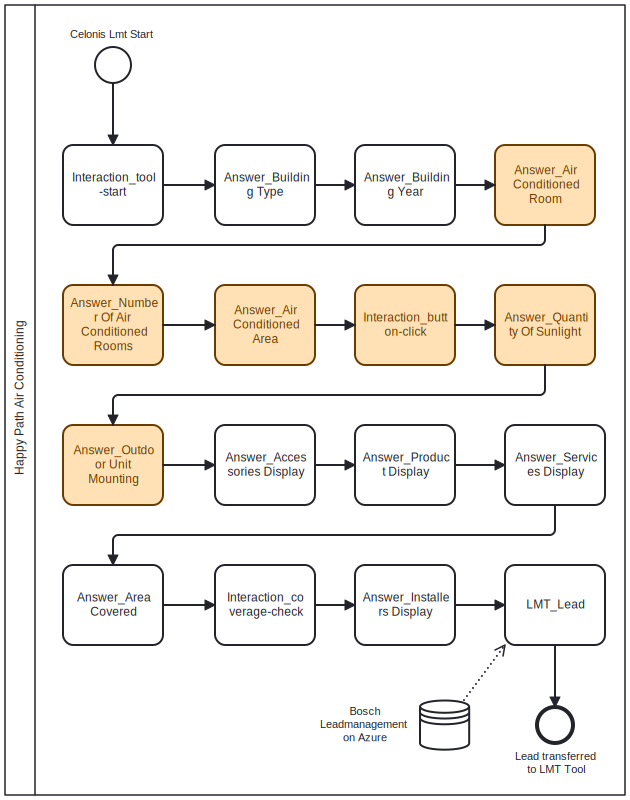
\includegraphics[width=0.8\linewidth]{images/bpmn/Wizard_Happy_Path_AirConditioning_Pool.pdf}
    \caption{Happy Path of Wizard data}
    \label{fig_happy_path_wizard}
\end{figure}


Figure \ref{fig_happy_path_wizard} shows the ``happy path'', meaning the most frequent trace of Wizard Data of the german Bosch homepage. As most leads were created for air conditioning technology, this trace represents a air conditioning flow. Therefore, there are some specific questions (e.g. area of placement of outdoor unit) to AC, which are highlighted yellow. 
Particularly noteworthy is that the first event is not \textit{Answer\_DesiredProduct}. This indicates that most leads did \textbf{not} originate from the general landing page but were instead initiated via product-specific sub-pages, such as those linked from social-media campaigns or similar channels.

\newpage
A complete process model of every possible technology selection can be seen inside the appendix in figure \ref{fig:wizard_flow_all_paths}. This model represents the ten most frequent variants, as well as specifically the trace for hybrid solutions (as they are selected very rarely and are not even part of the ten most frequent variants). It becomes clear that air conditioning traces differ a lot from traditional heating-only variants. E.g. the hybrid flow only differs in two question from a traditional ``heat pump'' flow, namely the events \textit{Answer\_Add\_Or\_New\_Hybrid} and \textit{Answer\_EnergySource\_Choices\_Hybrid}. The process chart in figure \ref{fig:wizard_flow_all_paths} covers \textbf{83\%} of all variants, meeting the requirements of \citeauthor{AalstSpaghetti} in chapter \ref{sec:lasagneshaphetti}.

A limitation from the Google Analytics dataset becomes visible in figure \ref{fig:wrong_modeling_wizard}. Sometimes, the next question shown inside the Wizard depends on the answer that was given in the previous question. However, this cannot be modeled by the heuristic miner inside Celonis. Either manual changes to the model have to be made or the selected answer must also be part of the event. Therefore, one could e.g. combine question and answer to distinguish between the traces of different selected models.

\begin{figure}
    \centering
    \includegraphics[width=0.9\linewidth]{images/bpmn/Incorrect_Modelling_Wizard.pdf}
    \caption{Wrong Modeling by Heuristic Miner}
    \label{fig:wrong_modeling_wizard}
\end{figure}

\newpage
\subsection{Lead Management Data}


As the dataset from the Lead Management Tool is way more complex, the control flow model is also looking more complex than the one from the Wizard data. In total, Celonis' Variant Explorer shows more than $2.000$ different variants of execution inside the log. For example, figure \ref{fig:lmt_modeling_5_frequent_variants} shows the control flow model with the five most frequent variants, figure \ref{fig:lmt_modeling_8_frequent_variants}  with the eight most frequent variants in comparison, growing rapidly in size. This model covers only \textbf{$31\%$} of all traces, therefore we can say that it does not meet the quality criteria of Section 2. Even by modeling only one installer (namely the one who sold the lead) instead of all potential three, no fitness above $80\%$ was achieved. While including additional variants marginally improves fitness, it also leads to a much larger increase in model complexity. Following the principle of Occam’s razor (see figure \ref{fig:four_quality_dimensions}), further expansion of the control-flow model is not beneficial and therefore stopped.


A combined version of both the Wizard data as well as the \ac{lmt} data with the eight most frequent variants can be seen in figure \ref{fig:wizard_lmt_combined} inside the appendix. High resolution source files are available inside a GitHub Repository, see chapter \ref{github} for further information.

\begin{figure}
    \centering
    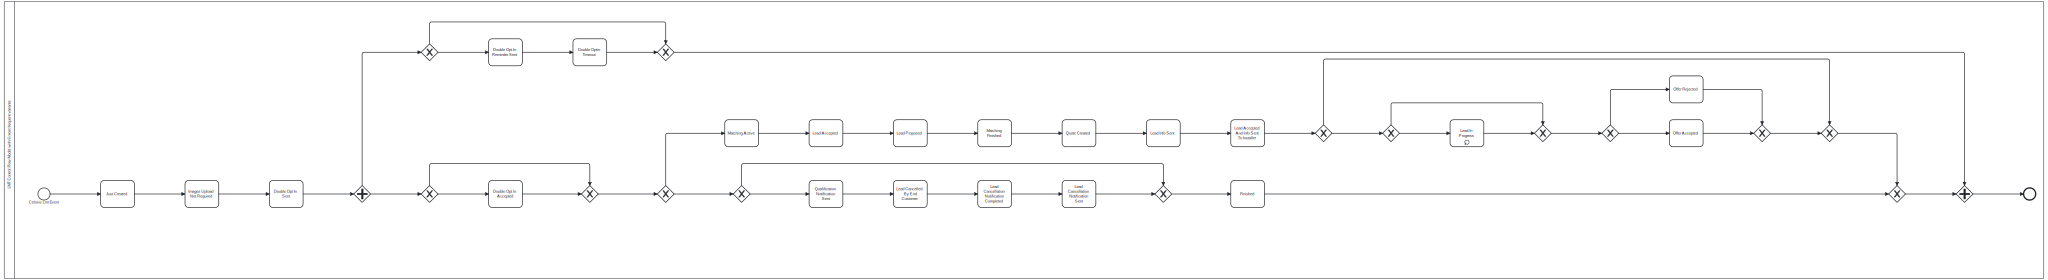
\includegraphics[width=1.0\linewidth]{images/bpmn/LMT_5_Variants.pdf}
    \caption{LMT Control Flow Model with 5 most frequent variants}
    \label{fig:lmt_modeling_5_frequent_variants}
\end{figure}

\begin{figure}
    \centering
    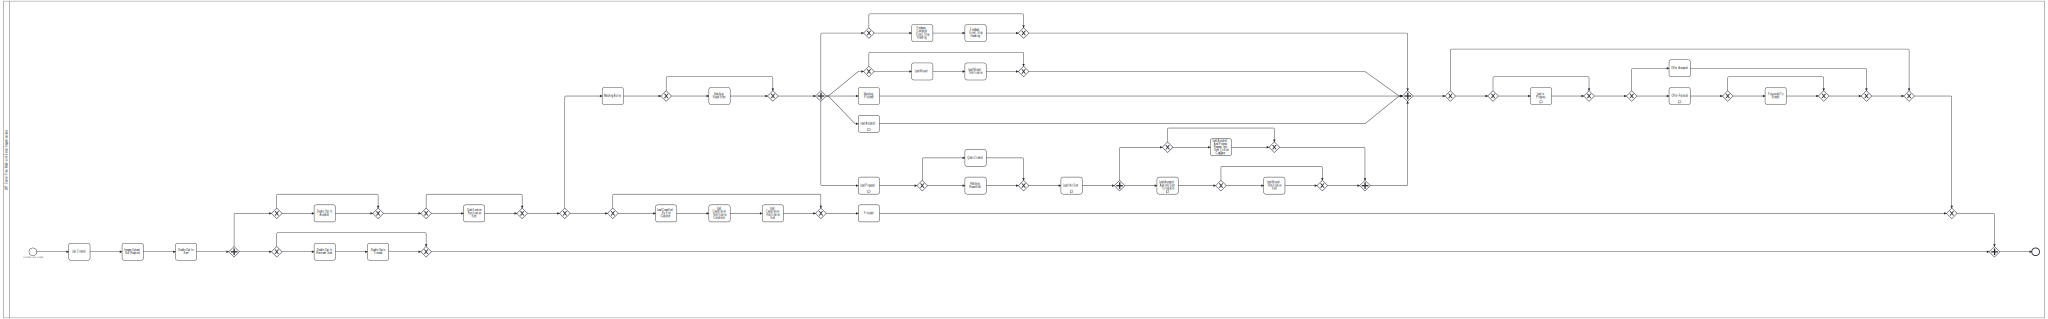
\includegraphics[width=1.0\linewidth]{images/bpmn/LMT_8_Variants.pdf}
    \caption{LMT Control Flow Model with 8 most frequent variants}
    \label{fig:lmt_modeling_8_frequent_variants}
\end{figure}


\clearpage
\section{Create Integrated Process Model}

These issues can be addressed during the creation of the integrated process model. In this step, \citeauthor{AalstSpaghetti} recommends refining the model not only structurally but also by incorporating organizational, temporal, and case-related information \cite{AalstSpaghetti}.

\textbf{Organizational Perspective} \\
One way of displaying the organizational perspective is the conversation model shown in figure \ref{fig:lmt_communication_diagram}. It shows the communication steps between different organizational units which are involved in the process, focusing on the exchange of information between the involved parties: \textit{Prospect}, \textit{Marketing Department}, \textit{Sales Department}, \textit{Installer}, and \textit{Customer}. This diagram highlights the sequence of communication events without describing the internal decision logic or the exact activity flow. It shows how a lead is initiated by the prospect, transferred to the marketing department for qualification, and subsequently forwarded to the sales department, which then engages with installers. Once an installer provides the product or service, the prospect transforms into a customer.

\begin{figure}
    \centering
    \includegraphics[width=1.0\linewidth]{images/bpmn/Lead Process Organizational View_cropped_cropped.pdf}
    \caption{Lead Management Conversation Model}
    \label{fig:lmt_communication_diagram}
\end{figure}

\newpage
\textbf{Time Perspective} \\
The duration of process execution is strongly influenced by chosen technology, involved installers and the end customer. External factors (such as governmental subsidies, which are beyond the control of Bosch) play a significant  role. Consequently, no explicit temporal perspective has been programmed into the current version of lead management at Bosch. The only time-related aspect considered is a lead timeout, which triggers if a lead is not accepted by any installer within 15 working days. Recommendations regarding the specification of lead timeouts and the integration of a more comprehensive temporal perspective are discussed in the conclusion of this work. 

\textbf{Case Perspective} 

The case perspective of the lead management process can be seen in figure \ref{fig:lmt_case_perspective}. The process begins when a prospect visits the website and initiates the lead wizard. Depending on the chosen technology, especially whether a heat pump is selected, the lead management tool triggers different qualification logic within the marketing department. Following the completion of the online questionnaire, the marketing-qualified lead is forwarded to sales, where installer selection is initiated. The process model further differentiates between cases in which prospects select installers themselves and cases in which the system automatically proposes the closest installers. As described in the text, up to three installers are notified simultaneously, and the two fastest respondents have the opportunity to accept the lead.

\begin{figure}[h!]
    \centering
    \includegraphics[width=1.0\linewidth]{images/bpmn/Process_Chart_cropped.pdf}
    \caption{Lead Management Case Perspective}
    \label{fig:lmt_case_perspective}
\end{figure}

\newpage
\section{Support}
This chapter focuses on using real-time data from running cases to detect deviations, predict future outcomes (e.g., remaining processing time), and recommend actions based on historical data. The results can be delivered directly to end users \cite{AalstSpaghetti}.

\subsection{Further Development}
Since the Lead Management Tool is constantly being changed and new features are added, the integrated process model needs to be updated frequently. Solution to this problem could be a \textbf{time filter} of attribute "createdAt". Since the current models are built on top of an event log reaching back to 1$^{st}$ of January 2024, it allows behavior that will not happen in new leads. For example, there is an event called \textit{DAAQualificationSent} that was removed in November 2024 and is not relevant in conformance checking of new leads. At max, it should only appear in old process models of 2024. 

\subsection{Alerting}
Celonis offers notification and alerting functions inside the \ac{pam}. This means, near to real time Celonis can check for deviations and contact colleagues. This could either be an option for developers to check for functional deviations, or for operational support (e.g. one lead stays too long in one specific status).

\subsection{Ownership}
As this proof of concept was build by german sales division, it cannot be maintained by a sales department since it exceeds their responsibilities. Therefore it will be passed on to \ac{bdo} who will roll out the Celonis Dashboard for every country that participates in Lead Management. \ac{bdo} will also ensure centralized governance, ongoing maintenance, and consistent data quality across regions. 


\chapter{Insights and Improvements}
This chapter is supposed to answer the questions that were made during chapter \ref{sec:question}. The following questions are either answered through Discovery, Variant Explorer or \ac{pql} formulas  made up as \ac{kpi} inside the knowledge model of Celonis.

\section{Lead Creation}

\textit{Q1. Is there a specific lead path, which most of the users go through while creating a lead?}

This question can be answered through the Celonis Variant Explorer. The happy path of the wizard data can be seen in figure \ref{fig_happy_path_wizard} which shows the trace of air conditioning leads, since they were requested the most by prospects. Second most frequent variant are leads for heat pumps, which are included in figure \ref{fig:wizard_flow_all_paths} as well as the technologies "hybrid", "gas" and "oil". As the sequence of questions can differ from the source URL and selected answers, the coverage of the nine most frequent variants acceptable with around $80\%$ (see table \ref{tab:variant-explorer}).

\begin{table}[h]
\centering
\begin{tabular}{l | l | l | l }
\textbf{Variant} & \textbf{Count} & \textbf{Coverage} & \textbf{Average TPT} \\
\hline
$\#1$ & $15{.}060$ & $24.6\%$ & $49 s$ \\
\hline
$\#2$ & $8{.}820$ & $14.4\%$ & $1 min$ \\
\hline
$\#3$ & $5{.}940$ & $12.3\%$ & $35 s$ \\
\hline
$\#4$ & $4{.}990$ & $10.3\%$ & $44 s$ \\
\hline
$\#5$ & $4{.}440$ & $6.2\%$ & $1 min$ \\
\hline
$\#6$ & $4{.}040$ & $4.1\%$ & $38 s$ \\
\hline
$\#7$ & $3{.}410$ & $4.1\%$ & $50 s$ \\
\hline
$\#8$ & $3{.}320$ & $2.0\%$ & $2 min$ \\
\hline
$\#9$ & $2{.}940$ & $2.0\%$ & $59 s$ \\
\hline
$Others$ & $13{.}240$ & $20.0\%$ & $54 s$ \\
\hline
\end{tabular}
\caption{Most frequent process variants}
\label{tab:variant-explorer}
\end{table}

\textit{Q2. Do user stay very long at one question as they do not know what to answer?}

This can be analyzed through the Celonis Process Explorer. Since prospects may temporarily leave the browser tab (e.g., to attend to other activities), throughput times vary substantially between the mean and the median.
This difference is particularly shown for the transition from the first to the second question, as the wizard tool is launched automatically when the URL is opened. Consequently, the recorded time between the events \textit{Answer\_BuildingType} and \textit{Answer\_LeadPurpose} is approximately one hour on average, while the median duration is only four seconds. For this reason, the median throughput time is considered more representative and is used for further analysis.

The longest median time is observed on the question \textit{Answer\_ServicesDisplay} with 31 seconds, followed by \textit{Answer\_OutdoorUnitMounting} with 25 seconds. This can likely be described by the fact that the event \textit{Answer\_ServicesDisplay} presents a large amount of textual information, which prospects must first read before selecting one or more desired services or explicitly choosing none. Some of the services can be seen in figure \ref{fig:services_wizard}.

\begin{figure}
    \centering
    \includegraphics[width=0.6\linewidth]{images/Wizard_longest_Median.png}
    \caption{Longest Median of Process Explorer}
    \label{fig:median_answer_services_Displayed}
\end{figure}

\begin{figure}[h]
    \centering
    \includegraphics[width=1.0\linewidth]{images/Wizard_Services.png}
    \caption{Selectable Services of event "Answer\_ServicesDisplay"}
    \label{fig:services_wizard}
\end{figure}

The comparatively long median duration for the event \textit{Answer\_OutdoorUnitMounting} is unexpected, as this question is intended for informational purposes only. Prospects can select from the options \textit{balcony}, \textit{façade}, \textit{top floor}, and \textit{other}. 

However, the final decision regarding the placement of the outdoor unit is ultimately made by the installer. Additionally, there is a very high drop of rate at that event of $19\%$. Therefore it is suggested to\textbf{ remove} that question from the HAT. 

\textit{Q3. Is there a specific lead path, in which users start and in which most users exit the Lead Management (LMT)?}

This question can be answered by a combination of questions \textit{Q1} and \textit{Q2} via the Process Explorer. Most prospects ($33\%$) start the Lead Manageent with the event \textit{Answer\_BuidlingType} which indicates that the lead originated from social media, since the events \textit{Answer\_LeadPurpose} and \textit{Answer\_Technology} do not appear. The second most frequent entry point ($30\%$) is the event \textit{Answer\_LeadPurpose}, representing prospects who clicked on a product-specific sub-page (e.g., heat pumps) and afterwards started the tool. The other $27\%$ of prospects come from the general landing page of Bosch Home Comfort Germany, as they just clicked on "Individual Offer".

Highest Drop-Off rates can be seen after events \textit{Answer\_OutdoorUnitMounting} with $19\%$ of all traces that lead through this event being terminated, followed by \textit{Answer\_Transfer} (e.g. floor or wall heating) with $13\%$. The third-highest drop-off rate occurs at the event \textit{Answer\_ProductDisplay}, with $7\%$. All remaining events show comparatively low drop-off rates below $4\%$.

As lead qualification is performed at a later stage by the marketing department anyways, each lead is valuable at this early point in the process. Consequently, it is recommended to \textbf{redesign} questions associated with high drop-off rates in order to reduce early LMT leaving and enable a higher number of leads to be generated at the beginning of the process.
\\
\newpage
\section{Lead Matching}

\textit{Q1. Is there a coincidence overall from rejected/missed leads? Regarding
\begin{enumerate}[a)]
        \item Lead source
        \item Technology
        \item Lead use case
        \item Area
    \end{enumerate}
}

Since the status and potential success of a lead is based on multiple factors (such as personal fit between installer and prospect, timing, use case etc.), coincidences are hard to find. However, Celonis Views allow page wide filters based on attributes of the event log. Since the initial event log (compare table \ref{tab:features}) has a column called \textit{Status}, anomaly detection was performed on Status Levels ``LeadRejected'' and ``LeadMissed''. There is no difference in rejected/missed leads in terms of their lead source. 
Per Technology, it is noticeable that AirConditioning contains more leads which where missed and rejected. This again can be explained due to peak weeks in summer, where a high amount of leads could not be handled by installers. While excluding these weeks, all technologies have roughly the same percentage of rejected ($30\%$) and missed ($10\%$) leads. 

On both Status, there is no noticeable difference in areal distribution inside Germany. Bosch distributes Germany into ten different regions with different sizes and revenue. As Bosch is a south-western based company, traditionally lead management works best in the Stuttgart-region where the brand is well-known and trusted. Therefore the most rejected and missed leads are from the sales region of southern-west Germany (called 927), followed by the second-biggest region around Frankfurt (called 909). 

\newpage
\textit{Q2. How long does it take overall that a lead is accepted?} 

This question can be answered either through a Celonis component called ``Throughput Time Explore'' or via a \ac{pql} formula with the following code that basically describes the \ac{kpi} ``Time-to-First-Touch'' which was already presented in section \ref{sec:performance-metrics}.
\begin{lstlisting}[language=SQL]
AVG(
  CALC_THROUGHPUT(
    FIRST_OCCURRENCE['DoubleOptInAccepted'] TO
    FIRST_OCCURRENCE['LeadAccepted'],
    REMAP_TIMESTAMPS(
      "celonis_lmt"."EVENTDATE",
      HOURS
    )
  )
)
\end{lstlisting}

As figure \ref{fig:avg_tpt_LeadAccepted} shows, the average varies between $0$ to $1488$ hours. The average time is $52,1h$, the median time is $32,1h$ until a lead is accepted by the first installer. This broad discrepancy can vary based on multiple reasons, such as that leads are not sent to installers during the weekend, resulting in longer throughput times and some unattractive leads, which go through multiple matching rounds until they are first accepted. As Celonis clusters the columns in $16h$-intervals, one can clearly see that most leads are accepted during the first $16$ hours after creation.

\begin{figure}[h!]
    \centering
    \includegraphics[width=0.75\linewidth]{images/KPI_throughput_toAccept_average.png}
    \caption{Average Throughput Time to Event "LeadAccepted"}
    \label{fig:avg_tpt_LeadAccepted}
\end{figure}

\textit{Q3. How long does it take per technology until a lead is accepted?}

\begin{figure}[h!]
    \centering
    \includegraphics[width=1.0\linewidth]{images/KPI_throughput_toAccept_average_Technology.png}
    \caption{Average Throughput Time to Event "LeadAccepted" per Technology}
    \label{fig:avg_tpt_LeadAccepted_tech}
\end{figure}

Figure \ref{fig:avg_tpt_LeadAccepted_tech} shows the same time frame as figure \ref{fig:avg_tpt_LeadAccepted}, but this time plotted by requested technology. Warm water ($12,14h$) and  gas heating ($15,77h$) leads are accepted way faster than e.g. heat pump leads ($46,05h$). This could be explained by the fact that they require way less planning and are overall cheaper and faster to install. Heat pumps take the longest time until they are accepted, with $46,05h$  from created time to accepted time. Striking are throughput times of air conditioning leads. After research, this is again due to the fact that there were peak lead creation numbers during high temperature summer weeks, where installers could not handle all the leads and were late on accepting new ones.

\clearpage
\section{Lead InProgress}

\textit{Q1. How long does it take until a lead is set in progress?} 

Similar to \textit{Q3} of section Lead Matching, the analysis was done both through the component ``Throughput Time Explore'' and via a \ac{pql} formula with the following code:
\begin{lstlisting}[language=SQL]
AVG(
  CALC_THROUGHPUT(
    FIRST_OCCURRENCE['LeadAccepted'] TO
    FIRST_OCCURRENCE['LeadInProgress'],
    REMAP_TIMESTAMPS(
      "celonis_lmt"."EVENTDATE",
      HOURS
    )
  )
)
\end{lstlisting}

Figure \ref{fig:avg_tpt_InProgress} shows the distribution of throughput times between the first occurrence of the event \textit{DoubleOptInAccepted} and the last occurrence of \textit{LeadInProgress}. The average throughput time amounts to approximately $904$ hours, while the median is significantly lower at around $575$ hours, indicating a strongly right-skewed distribution.
Most leads are set in progress within the first few hundred hours, as reflected by the high frequency in the lower time bins. However, a considerable number of cases exhibit very long waiting times, with a maximum of more than $6.000$ hours. These long-running cases heavily influence the average and point towards process inefficiencies or exceptional situations such as missing resources or backlog accumulation. 

\begin{figure}
    \centering
    \includegraphics[width=0.75\linewidth]{images/KPI_throughput_toInProgress_average.png}
    \caption{Average Throughput Time to Event "InProgress"}
    \label{fig:avg_tpt_InProgress}
\end{figure}

\textit{Q2. How long does it take per technology until is set in progress?}

\begin{figure}
    \centering
    \includegraphics[width=1.0\linewidth]{images/KPI_throughput_toInProgress_average_Technology.png}
    \caption{Average Throughput Time to Event "InProgress" per Technology}
    \label{fig:avg_tpt_InProgress_Tech}
\end{figure}

Figure \ref{fig:avg_tpt_InProgress_Tech} displays the average throughput time from event \textit{DoubleOptInAccepted} to event \textit{LeadInProgress}, broken down by requested technology. Clear differences between technologies can be observed.
Air conditioning leads reach the in-progress status fastest with an average of approximately $115$ hours, followed by heat pump and warm water leads. 

Gas heating and hybrid technologies show noticeably longer throughput times, while oil heating exhibits the highest average duration at roughly $186$ hours. These differences can largely be explained by varying planning complexity and installation requirements. Technologies such as air conditioning or warm water typically are cheaper and require less technical coordination. In contrast,  hybrid systems and heat pumps often involve more complex evaluations.
Overall, the figure underlines that technology choice is a key driver of throughput time.

\textit{Q3. Are there leads which are never set in progress? And if so, why?}

To answer that question, traces, where the event \textit{LeadInProgress} did not appear need to be filtered out. This can be done either via page-wide filters to analyze the \ac{kpi}s mentioned in chapter \ref{sec:performance-metrics} and figure \ref{fig:celonis_landing_page} or via the Celonis Process Explorer shown in figure \ref{fig:celonis_process_explorer}. The Process Explorer shows clearly, that $28\%$ of all $12.000$ leads in 2025 never run through the event \textit{LeadInProgress}, meaning they are accepted but never a product is offered by at least one installer. $17\%$ of all leads end at this event, meaning Bosch does not know, whether a product is sold or not. After excluding this event and plotting the leads by create date, there are spikes during summer, indicating that one reason is again the high air conditioning amount during high temperature summer weeks. However, it is more likely that a heat pump lead is never set \textit{InProgress} than a air conditioning lead, as heat pumps are over represented. Also, the sales region around Dortmund (called ``921'') is over represented. Further research has to be taken to answer that question more clearly.

\begin{figure}
    \centering
    \includegraphics[width=0.9\linewidth]{images/Process_Explorer_LeadInProgress.png}
    \caption{Celonis Process Explorer}
    \label{fig:celonis_process_explorer}
\end{figure}

\newpage
\section{Lead Completion}

\textit{Q1. Which kind of leads are mostly sold / not sold overall?}

This question can be answered using one of the metrics introduced in chapter \ref{sec:performance-metrics}. Namely, the sales rate can be calculated in \ac{pql} with this formula:

\begin{lstlisting}[language=SQL]
AVG(
  CASE(
    WHEN "celonis_lmt"."EVENTDATE" = 'Sold'
    THEN 1.0 ELSE 0.0
    END
   )
)
\end{lstlisting}

After creating this \ac{kpi}, a desired direction (in this case upwards) needs to be declared. Celonis offers a feature called ``Insight Explorer'' which makes suggestions and calculates the affect of that change to the \ac{kpi}.
Some suggestions are: 

\newpage
\begin{enumerate}
    \item Changing the question regarding energy consumption to a mandatory field can boost the sales rate (special type of \ac{kpi} ``Conversion Rate'' in table \ref{tab:lead_process_kpis}) from $16,58\%$ to $18,06\%$. This would roughly result in a revenue growth of $1.400.000$ \euro, assuming total lead volume stays the same and \ac{lmt} is accountable for $20\%$ of all sales.
    \item As lead purpose ``New Build'' has a $8,1\%$ lower sales rate than others, a differentiated prioritization strategy may be considered.
    \item Building types ``flat'' and semi detached flat have a much lower probability of being sold compared to other building types, mainly detached and semi detached (compare figure \ref{fig:celonis_insight_explorer}).
    \item Air conditioning, gas- and oil heating (all around $16\%$) have a much higher sales rate than heat pumps ($11,27\%$).
\end{enumerate}

\begin{figure}
    \centering
    \includegraphics[width=1.0\linewidth]{images/Celonis_Insight_Explorer.png}
    \caption{Example Suggestions of Insight Explorer}
    \label{fig:celonis_insight_explorer}
\end{figure}

\textit{Q2. Which kind of leads are mostly sold / not sold from a specific installer?}

To answer this question, all measures and visuals create from the question above are added a dimension from the event log attributes called ``KUNNR'', representing the customer number of every installer. Sales rate differs very much by installer, also the distribution of building types, purpose and requested technology. This makes clear that installers have preferences. However its not clear why metrics such as sales rate, conversion rate or time-to-first touch differ that much from installer to installer. 

One explanation might be that some installers take Lead Management more seriously, make better offers, or are more polite towards end customers, resulting in more sales.

\textit{Q3. Which installers have the highest probability to get the lead done if it was forwarded after not matchable?}

This question aims towards an event called \textit{ForwardedToInstaller} which only occurs after manual admin action. First, a lead has to be missed after the first two matching rounds. Afterwards, it reaches it final status \textit{NotMatchable} where the end customer is notified, that no suitable installer was found. If an admin interferes with that status, the lead is again ``open'' and can be sent to other installers. In 2025, this has happened $224$ times of around $19.643$ leads in total. Of these $224$ leads, only $2$ were confirmed sales. Because of this, the question cannot be answered, as the sample size is too small and therefore will be considered in future work.